\documentclass[a4paper,11pt]{report}
\usepackage[utf8]{inputenc}
\usepackage[T1]{fontenc}
\usepackage{lmodern}
\usepackage[spanish,es-tabla]{babel}
\usepackage[margin=2.5cm]{geometry}
\usepackage{amsmath,amsfonts,amssymb}
\usepackage{booktabs}
\usepackage{multirow}
\usepackage{graphicx}
\usepackage{pdflscape}
\usepackage{float}
\usepackage{tabularx}
\usepackage{enumitem}
\usepackage[table]{xcolor}
\usepackage{adjustbox}
\providecommand{\euro}{€}
\usepackage{hyperref}
\hypersetup{
    colorlinks=true,
    linkcolor=blue!70!black,
    citecolor=blue!70!black,
    urlcolor=blue!70!black
}

\title{
\includegraphics[width=0.30\textwidth]{figuras/escudo.png}\\[1.0cm]
\Huge{\textbf{Estudio Económico y Financiero de una Planta de Producción}}\\[0.8em]
\LARGE{\textbf{Evaluación de Viabilidad, Flujos de Caja y Análisis de Sensibilidad Multidimensional}}\\[0.5em]
\large\textit{Seminario de Organización y Gestión de Proyectos --- Curso 2026/2027}}

\author{\Large\textbf{Christian Pérez Hita}\\[0.4em]
\normalsize Grado en Ingeniería Química --- Universidad de Granada (UGR)\\[0.2em]
\normalsize Parámetro de asignación: $AB = 19$}

\date{Noviembre de 2026}

\begin{document}

\maketitle

\begin{abstract}
En este documento se desarrolla el estudio económico-financiero para la implantación y puesta en marcha de una planta industrial de producción química con un horizonte de explotación proyectado a 20 años. Siguiendo la metodología del Seminario de Presupuestos de la asignatura \textit{Organización y Gestión de Proyectos}, el análisis se plantea en dos bloques complementarios: por un lado, el estudio de la \textbf{viabilidad económica intrínseca del proyecto} (evaluando el rendimiento puro de los activos productivos sin considerar deuda) y, por otro, el estudio de la \textbf{viabilidad financiera desde la óptica del inversor promotor} (incorporando una financiación ajena del 49,50\% mediante un préstamo bancario a 10 años amortizado por el sistema francés a un tipo de interés fijo del 7,00\% anual).

A partir de los parámetros individuales asignados según el dígito de control ($AB = 19$), la planta se diseña para una capacidad nominal de 9,19~t/día durante 289 días de operación anual (2.655,91~t/año), con un precio de venta en fábrica de 1,019~\euro/kg, lo que supone una facturación anual constante de 2.706.372,29~\euro/año. Frente a una inversión inicial en inmovilizado material de 7.615.000,00~\euro{} y unos gastos operativos anuales de 1.329.300,00~\euro/año (que arrojan un EBITDA de 1.377.072,29~\euro/año), los resultados confirman una rentabilidad holgada en ambos escenarios. Actualizando los flujos a la tasa de descuento de referencia del 5,00\%, el proyecto presenta un Valor Actual Neto (VAN) de 6.558.463,97~\euro, una Tasa Interna de Retorno (TIR) del 13,97\% y un Periodo de Recuperación de la Inversión (PRI) de 6,58 años. Desde la perspectiva de los accionistas, el apalancamiento financiero positivo impulsa la TIR de los recursos propios hasta el 18,55\%, con un VAN del inversor de 6.511.628,24~\euro{} y un plazo de recuperación de 5,71 años.

Por último, el estudio incorpora un análisis de sensibilidad frente a la tasa de descuento (entre el 0\% y el 30\%) y frente a desviaciones del $\pm 10\%$ en las variables operativas clave (precio de venta, volumen de producción y coste de materia prima), determinando analíticamente los umbrales críticos de rentabilidad que anularían el VAN del proyecto.
\end{abstract}

\tableofcontents
\newpage

\chapter{Introducción, Objeto y Metodología}

\section{Objeto del Estudio}
El objetivo de este informe es determinar de manera cuantitativa si la inversión necesaria para construir y operar una planta química industrial de 2.655,91~t/año resulta rentable y financieramente sostenible a lo largo de una vida útil de 20 años. En cualquier proyecto de ingeniería química, el dimensionamiento de los equipos y el cierre de los balances de materia y energía deben ir acompañados de una validación económica que responda a cuatro cuestiones prácticas:
\begin{enumerate}[label=\alph*)]
    \item Comprobar si los activos productivos de la planta son capaces de generar por sí mismos un flujo de caja suficiente para recuperar el desembolso inicial y superar el coste de oportunidad del capital ($k = 5,00\%$).
    \item Evaluar el rendimiento específico que obtienen los promotores sobre el capital propio aportado tras atender el servicio de la deuda bancaria.
    \item Verificar que la tesorería anual de la planta permite cubrir sin tensiones las cuotas de amortización e intereses del préstamo durante los primeros diez años de explotación.
    \item Cuantificar el margen de seguridad del proyecto ante posibles caídas en el precio de venta o en el ritmo de producción, así como ante encarecimientos de la materia prima.
\end{enumerate}

\section{Metodología de Evaluación y Diferenciación Conceptual}
De acuerdo con el planteamiento del seminario y con el modelo de cálculo desarrollado en el libro de hojas de cálculo adjunto (\path{Estudio_Economico_Financiero_Christian_Perez_Hita.xlsx}), el análisis distingue claramente entre la rentabilidad del activo y la rentabilidad del accionista:
\begin{itemize}
    \item \textbf{Estudio Económico de la Planta (Perspectiva del Proyecto Puro):} Analiza el rendimiento técnico-económico de la instalación como si se financiase íntegramente con capital propio ($I_0 = 7.615.000,00\text{ \euro}$). No se deducen intereses ni devoluciones de principal bancario, de modo que el resultado depende exclusivamente de la eficiencia operativa de la planta. El Flujo Neto de Caja anual del proyecto ($FNC_{\text{proy},t}$) se obtiene sumando de nuevo la amortización contable al beneficio neto después de impuestos, dado que la depreciación es un apunte contable que no supone salida real de dinero:
    \begin{equation}\label{eq:fnc_proyecto}
    \begin{aligned}
        FNC_{\text{proy},t} &= \text{EBITDA}_t - \text{Amort}_t - \text{IS}_{\text{proy},t} + \text{Amort}_t \\
        &= (\text{EBITDA}_t - \text{Amort}_t)\cdot(1 - t_{\text{IS}}) + \text{Amort}_t = \text{BN}_{\text{proy},t} + \text{Amort}_t
    \end{aligned}
    \end{equation}
    \item \textbf{Estudio Financiero del Inversor (Perspectiva de los Recursos Propios):} Evalúa los flujos de caja que quedan a disposición de los socios tras incorporar el préstamo bancario por el 49,50\% de la inversión inicial ($3.769.425,00\text{ \euro}$), reduciendo el desembolso inicial propio en $t=0$ a $3.845.575,00\text{ \euro}$. Durante los primeros 10 años, los intereses anuales de la deuda ($I_t$) se restan antes de calcular el Impuesto sobre Sociedades ($t_{\text{IS}} = 25\%$), generando un ahorro o escudo fiscal igual a $t_{\text{IS}}\cdot I_t$, mientras que la devolución anual del principal ($\Delta D_t$) se descuenta directamente del flujo de caja tras impuestos:
    \begin{equation}\label{eq:fnc_inversor}
    \begin{aligned}
        FNC_{\text{inv},t} &= (\text{EBITDA}_t - \text{Amort}_t - I_t)\cdot(1 - t_{\text{IS}}) + \text{Amort}_t - \Delta D_t \\
        &= \text{BN}_{\text{inv},t} + \text{Amort}_t - \Delta D_t = FNC_{\text{proy},t} - I_t\cdot(1 - t_{\text{IS}}) - \Delta D_t
    \end{aligned}
    \end{equation}
\end{itemize}

\chapter{Bases de Diseño y Parametrización de la Planta}

\section{Asignación de Parámetros Individuales (\texorpdfstring{$AB = 19$}{AB = 19})}
Siguiendo el enunciado del seminario, los datos de partida de capacidad, precio de venta y estructura de capital quedan fijados a partir de las dos últimas cifras del DNI del autor ($AB = 19$):
\begin{itemize}
    \item \textbf{Capacidad diaria de producción nominal ($q_{\text{prod}}$):}
    \begin{equation}
        q_{\text{prod}} = 9 + \frac{AB}{100} = 9 + \frac{19}{100} = 9,19\text{ t/día} \quad (9.190\text{ kg/día})
    \end{equation}
    Operando durante un régimen industrial de 289 días efectivos al año (descontando paradas programadas de mantenimiento y limpieza), la producción anual comercializable asciende a:
    \begin{equation}
        Q_{\text{anual}} = 9,19\text{ t/día} \times 289\text{ días/año} = 2.655,91\text{ t/año} \quad (2.655.910\text{ kg/año})
    \end{equation}
    \item \textbf{Precio de venta unitario del producto terminado ($p_{\text{venta}}$):}
    \begin{equation}
        p_{\text{venta}} = 1,0 + \frac{AB}{1000} = 1,0 + \frac{19}{1000} = 1,019\text{ \euro/kg} \quad (1.019,00\text{ \euro/t})
    \end{equation}
    \item \textbf{Proporción de financiación ajena sobre la inversión inicial ($\%_{\text{deuda}}$):}
    \begin{equation}
        \%_{\text{deuda}} = 40 + \frac{AB}{2} = 40 + \frac{19}{2} = 49,50\%
    \end{equation}
    \item \textbf{Proporción de recursos propios aportados por los promotores ($\%_{\text{propio}}$):}
    \begin{equation}
        \%_{\text{propio}} = 100\% - \%_{\text{deuda}} = 100\% - 49,50\% = 50,50\%
    \end{equation}
\end{itemize}

\section{Inversión en Activos Fijos y Periodos de Amortización}
La inversión inicial requerida para la implantación de la planta asciende a 7.615.000,00~\euro{} (celda \texttt{B16} de la hoja \texttt{Resumen}), distribuida en tres partidas de inmovilizado material que se amortizan linealmente sin valor residual a lo largo de su vida útil contable:

\begin{table}[H]
\centering
\caption{Inversión inicial requerida en activos fijos y cuadro de amortización contable lineal.}
\label{tab:inversion_activos}
\small
\renewcommand{\arraystretch}{1.24}
\setlength{\tabcolsep}{7pt}
\adjustbox{max width=\textwidth}{%
\begin{tabular}{@{}lrrrr@{}}
\toprule
\textbf{Partida de Inversión} & \textbf{\shortstack[r]{Coste Inicial\\(\euro)}} & \textbf{\shortstack[r]{Peso s/ Total\\(\%)}} & \textbf{\shortstack[r]{Vida Útil\\(Años)}} & \textbf{\shortstack[r]{Cuota Anual\\(\euro/año)}} \\
\midrule
Obra Civil y Edificaciones & 1.000.000,00 & 13,13\% & 20 & 50.000,00 \\
Instalaciones Auxiliares e Informática & 115.000,00 & 1,51\% & 10 & 11.500,00 \\
Maquinaria Principal de Proceso (A) & 6.500.000,00 & 85,36\% & 15 & 433.333,33 \\
\midrule
\textbf{Total Inmovilizado Material ($I_0$)} & \textbf{7.615.000,00} & \textbf{100,00\%} & --- & \textbf{494.833,33}$^*$ \\
\bottomrule
\end{tabular}}
\vspace{0.4em}
\par\noindent\footnotesize{\textit{Nota ($^*$):} Debido a los distintos horizontes de depreciación de cada activo, la dotación conjunta de amortización presenta tres escalones a lo largo del proyecto: en los \textbf{años 1 a 10} asciende a \textbf{494.833,33~\euro/año} ($50.000 + 11.500 + 433.333,33$); en los \textbf{años 11 a 15}, una vez amortizadas por completo las instalaciones de 10 años, se sitúa en \textbf{483.333,33~\euro/año} ($50.000 + 433.333,33$); y en los \textbf{años 16 a 20}, extinguida ya la vida contable de la maquinaria principal, queda únicamente la cuota de la obra civil de \textbf{50.000,00~\euro/año}.}
\end{table}

\begin{figure}[H]
\centering
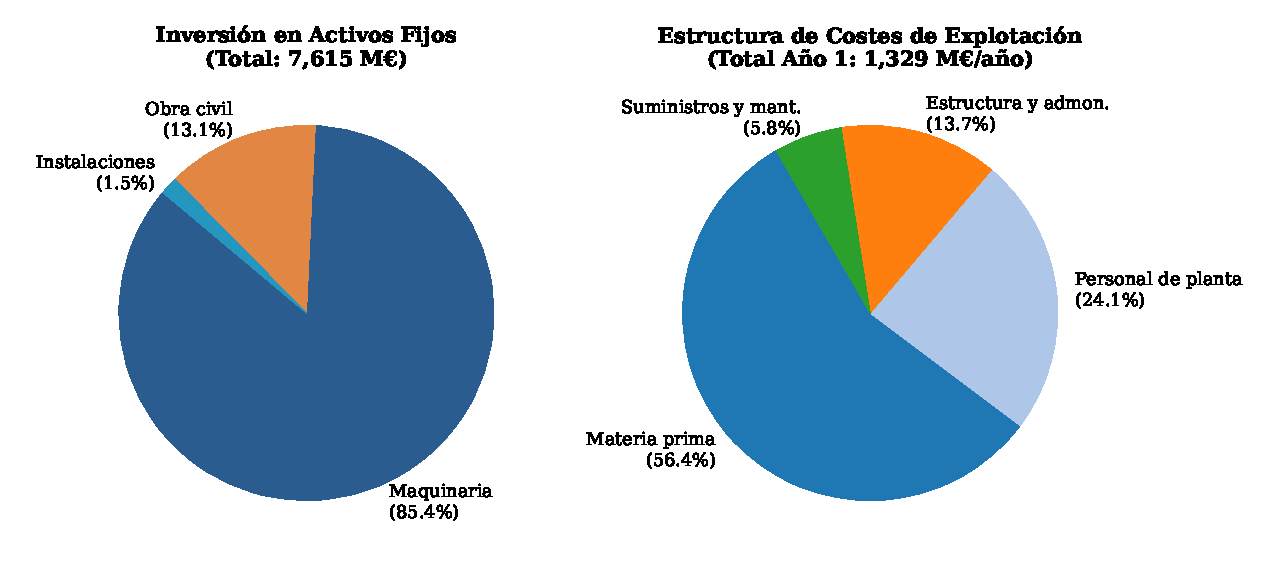
\includegraphics[width=0.90\textwidth]{figuras/distribucion_costes_inversion.pdf}
\caption{Distribución porcentual del presupuesto de inversión inicial (CAPEX) y de la estructura de costes de explotación (OPEX).}
\label{fig:distribucion_costes}
\end{figure}

\chapter{Costes de Explotación, Ingresos y Financiación}

\section{Estructura de Gastos de Explotación y Plantilla}
Para dotar de total trazabilidad al cálculo del margen operativo, en la hoja \texttt{Resumen} del libro de Excel (bloques 2 y 3, columnas \texttt{E:J}) se ha desglosado partida a partida el presupuesto anual de gastos de explotación (OPEX), que asciende a \textbf{1.329.300,00~\euro/año} y se vincula directamente con la celda \texttt{B29}. Los costes operativos se dividen en costes directos de fabricación (86,35\% del total) y gastos indirectos o de estructura (13,65\%):

\begin{table}[H]
\centering
\caption{Desglose detallado de los gastos anuales de explotación (OPEX).}
\label{tab:costes_operativos}
\small
\renewcommand{\arraystretch}{1.24}
\setlength{\tabcolsep}{6pt}
\adjustbox{max width=\textwidth}{%
\begin{tabular}{@{}llrr@{}}
\toprule
\textbf{Partida / Concepto de Coste Operativo} & \textbf{Desglose Técnico en Modelo Excel} & \textbf{\shortstack[r]{Importe Anual\\(\euro/año)}} & \textbf{\shortstack[r]{Peso\\(\%)}} \\
\midrule
\multicolumn{4}{@{}l}{\textbf{\textit{A. Gastos Directos de Fabricación}}} \\
A.1. Materia prima de proceso & Aprovisionamiento anual de proceso & 750.000,00 & 56,42\% \\
A.2. Transporte y embalaje & Transporte ($10.000\text{ \euro}$) + Embalaje ($50.000\text{ \euro}$) & 60.000,00 & 4,51\% \\
A.3. Mano de obra directa de planta & 12 efectivos de fábrica y laboratorio (\texttt{=I26}) & 320.000,00 & 24,07\% \\
A.4. Suministros industriales & Agua ($2.500\text{ \euro}$) + Gas ($2.800\text{ \euro}$) + Elec. ($6.500\text{ \euro}$) & 11.800,00 & 0,89\% \\
A.5. Mantenimiento y reparación & Conservación preventiva y correctiva de equipos & 6.000,00 & 0,45\% \\
\midrule
\textbf{Subtotal A --- Gastos Directos} & \textbf{Suma de partidas A.1 a A.5 (\texttt{=SUMA(I6:I10)})} & \textbf{1.147.800,00} & \textbf{86,35\%} \\
\midrule
\multicolumn{4}{@{}l}{\textbf{\textit{B. Gastos Indirectos y de Estructura General}}} \\
B.1. Personal de admon. y estructura & 5 efectivos de gerencia y admon. (\texttt{=I30}) & 140.000,00 & 10,53\% \\
B.2. Material de oficina e informática & Equipos, licencias de software y consumibles & 40.000,00 & 3,01\% \\
B.3. Comunicaciones y conectividad & Telefonía fija, móvil e internet industrial & 1.500,00 & 0,11\% \\
\midrule
\textbf{Subtotal B --- Gastos Indirectos} & \textbf{Suma de partidas B.1 a B.3 (\texttt{=SUMA(I12:I14)})} & \textbf{181.500,00} & \textbf{13,65\%} \\
\midrule
\textbf{TOTAL GASTOS DE EXPLOTACIÓN} & \textbf{OPEX Anual = Subtotal A + Subtotal B (\texttt{B29})} & \textbf{1.329.300,00} & \textbf{100,00\%} \\
\bottomrule
\end{tabular}}
\end{table}

El coste total de personal (460.000,00~\euro/año, que representa el 34,60\% de los gastos de explotación) procede de una plantilla de 17 trabajadores organizada en dos bloques funcionales, tal y como se recoge en la Tabla~\ref{tab:plantilla}:

\begin{table}[H]
\centering
\caption{Detalle de la plantilla laboral de la empresa e imputación en la estructura de costes.}
\label{tab:plantilla}
\small
\renewcommand{\arraystretch}{1.24}
\setlength{\tabcolsep}{6.5pt}
\adjustbox{max width=\textwidth}{%
\begin{tabular}{@{}lcrrl@{}}
\toprule
\textbf{Puesto / Categoría Profesional} & \textbf{Efectivos} & \textbf{\shortstack[r]{Coste Unitario\\(\euro/año)}} & \textbf{\shortstack[r]{Coste Total\\(\euro/año)}} & \textbf{\shortstack[l]{Imputación en\\Gastos OPEX}} \\
\midrule
Químico de Laboratorio & 1 & 40.000,00 & 40.000,00 & Directo (Partida A.3) \\
Ingenieros de Producción & 2 & 35.000,00 & 70.000,00 & Directo (Partida A.3) \\
Personal de Mantenimiento & 2 & 30.000,00 & 60.000,00 & Directo (Partida A.3) \\
Personal de Almacén & 2 & 30.000,00 & 60.000,00 & Directo (Partida A.3) \\
Trabajadores de Planta (Operarios) & 5 & 18.000,00 & 90.000,00 & Directo (Partida A.3) \\
\midrule
\textbf{Subtotal Mano de Obra Directa (A.3)} & \textbf{12} & --- & \textbf{320.000,00} & \textbf{Pasa a celda \texttt{I8}} \\
\midrule
Gerencia General & 1 & 60.000,00 & 60.000,00 & Indirecto (Partida B.1) \\
Personal Administrativo & 2 & 25.000,00 & 50.000,00 & Indirecto (Partida B.1) \\
Personal de Limpieza & 2 & 15.000,00 & 30.000,00 & Indirecto (Partida B.1) \\
\midrule
\textbf{Subtotal Personal de Estructura (B.1)} & \textbf{5} & --- & \textbf{140.000,00} & \textbf{Pasa a celda \texttt{I12}} \\
\midrule
\textbf{TOTAL PLANTILLA DE LA EMPRESA} & \textbf{17} & --- & \textbf{460.000,00} & \textbf{34,60\% del OPEX} \\
\bottomrule
\end{tabular}}
\end{table}

\section{Estructura de Financiación y Préstamo Francés}
Atendiendo a los coeficientes de estructura financiera derivados de $AB = 19$, el desembolso inicial de $I_0 = 7.615.000,00\text{ \euro}$ se cubre mediante:
\begin{itemize}
    \item \textbf{Préstamo bancario a largo plazo ($49,50\%$):}
    \begin{equation}
        P_{\text{deuda}} = 7.615.000,00\text{ \euro} \times 0,495 = 3.769.425,00\text{ \euro}
    \end{equation}
    \item \textbf{Aportación de recursos propios de los socios ($50,50\%$):}
    \begin{equation}
        E_{\text{propio}} = 7.615.000,00\text{ \euro} \times 0,505 = 3.845.575,00\text{ \euro}
    \end{equation}
\end{itemize}

El préstamo bancario se concierta a un plazo de $n = 10\text{ años}$ con un tipo de interés nominal fijo del $i_{\text{deuda}} = 7,00\%$ anual y amortización por el \textbf{sistema francés} de anualidad constante ($a$). Aplicando la fórmula de actualización de rentas constantes (equivalente a la función \texttt{PAGO(7\%; 10; -3769425)} en la celda \texttt{B23} de \texttt{Resumen} y \texttt{C4} de \texttt{Prestamo}), la cuota anual total a satisfacer al banco resulta:
\begin{equation}
    a = P_{\text{deuda}} \cdot \frac{i_{\text{deuda}}(1+i_{\text{deuda}})^n}{(1+i_{\text{deuda}})^n - 1} = 3.769.425,00 \cdot \frac{0,07\cdot(1,07)^{10}}{(1,07)^{10} - 1} = 536.681,32\text{ \euro/año}
\end{equation}

En cada ejercicio $t \in \{1,\dots,10\}$, los intereses devengados se calculan aplicando el 7,00\% sobre el saldo vivo al inicio del año ($I_t = 0,07 \cdot C_{t-1}$), destinándose la diferencia hasta completar la anualidad constante a amortizar principal ($\Delta D_t = a - I_t$). En la Tabla~\ref{tab:cuadro_prestamo} se presenta el cuadro de amortización completo obtenido en la hoja \texttt{Prestamo}:

\begin{table}[H]
\centering
\caption{Cuadro de amortización del préstamo bancario (Sistema Francés, 10 años, interés fijo del 7,00\%).}
\label{tab:cuadro_prestamo}
\small
\renewcommand{\arraystretch}{1.22}
\setlength{\tabcolsep}{6.5pt}
\adjustbox{max width=\textwidth}{%
\begin{tabular}{@{}crrrrr@{}}
\toprule
\textbf{Año} & \textbf{\shortstack[r]{Deuda Viva\\Inicial (\euro)}} & \textbf{\shortstack[r]{Cuota Anual\\Constante (\euro)}} & \textbf{\shortstack[r]{Intereses\\Pagados (\euro)}} & \textbf{\shortstack[r]{Capital\\Amortizado (\euro)}} & \textbf{\shortstack[r]{Deuda Viva\\Final (\euro)}} \\
\midrule
1  & 3.769.425,00 & 536.681,32 & 263.859,75 & 272.821,57 & 3.496.603,43 \\
2  & 3.496.603,43 & 536.681,32 & 244.762,24 & 291.919,08 & 3.204.684,35 \\
3  & 3.204.684,35 & 536.681,32 & 224.327,90 & 312.353,41 & 2.892.330,94 \\
4  & 2.892.330,94 & 536.681,32 & 202.463,17 & 334.218,15 & 2.558.112,79 \\
5  & 2.558.112,79 & 536.681,32 & 179.067,90 & 357.613,42 & 2.200.499,36 \\
6  & 2.200.499,36 & 536.681,32 & 154.034,96 & 382.646,36 & 1.817.853,00 \\
7  & 1.817.853,00 & 536.681,32 & 127.249,71 & 409.431,61 & 1.408.421,39 \\
8  & 1.408.421,39 & 536.681,32 & 98.589,50  & 438.091,82 & 970.329,57 \\
9  & 970.329,57   & 536.681,32 & 67.923,07  & 468.758,25 & 501.571,33 \\
10 & 501.571,33   & 536.681,32 & 35.109,99  & 501.571,33 & 0,00 \\
\midrule
\textbf{TOTAL} & --- & \textbf{5.366.813,18} & \textbf{1.597.388,18} & \textbf{3.769.425,00} & \textbf{0,00} \\
\bottomrule
\end{tabular}}
\end{table}

\chapter{Cuenta de Resultados y Flujos Netos de Caja}

\section{Cuenta de Resultados del Proyecto y del Inversor}
A partir de la producción anual nominal ($2.655.910\text{ kg/año}$) y del precio de venta en planta ($1,019\text{ \euro/kg}$), la facturación anual se mantiene constante a lo largo de los 20 años de operación:
\begin{equation}
    \text{Ingresos Anuales} = 2.655.910\text{ kg/año} \times 1,019\text{ \euro/kg} = 2.706.372,29\text{ \euro/año}
\end{equation}

Descontando los gastos anuales de explotación ($1.329.300,00\text{ \euro/año}$), se obtiene un resultado bruto de explotación (EBITDA) constante en todos los ejercicios:
\begin{equation}
    \text{EBITDA} = 2.706.372,29 - 1.329.300,00 = 1.377.072,29\text{ \euro/año}
\end{equation}

Sobre este margen bruto se aplica el esquema contable y fiscal recogido en la hoja \texttt{FlujosCaja} del modelo Excel:
\begin{enumerate}
    \item \textbf{Flujos Netos de Caja del Proyecto (Sin Deuda):} Al restar del EBITDA la dotación de amortización contable de cada tramo temporal y liquidar el Impuesto sobre Sociedades al $t_{\text{IS}} = 25\%$, se obtienen tres escalones de flujo neto de caja operativo según la Ecuación~\eqref{eq:fnc_proyecto}:
    \begin{itemize}
        \item \textbf{Años 1 a 10 ($\text{Amort} = 494.833,33\text{ \euro/año}$):} $\text{EBIT} = 882.238,96\text{ \euro/año}$, $\text{IS} = 220.559,74\text{ \euro/año}$, $\text{BN}_{\text{proy}} = 661.679,22\text{ \euro/año}$ y $\mathbf{FNC_{\text{proy}} = 1.156.512,55\text{ \euro/año}}$.
        \item \textbf{Años 11 a 15 ($\text{Amort} = 483.333,33\text{ \euro/año}$):} $\text{EBIT} = 893.738,96\text{ \euro/año}$, $\text{IS} = 223.434,74\text{ \euro/año}$, $\text{BN}_{\text{proy}} = 670.304,22\text{ \euro/año}$ y $\mathbf{FNC_{\text{proy}} = 1.153.637,55\text{ \euro/año}}$.
        \item \textbf{Años 16 a 20 ($\text{Amort} = 50.000,00\text{ \euro/año}$):} $\text{EBIT} = 1.327.072,29\text{ \euro/año}$, $\text{IS} = 331.768,07\text{ \euro/año}$, $\text{BN}_{\text{proy}} = 995.304,22\text{ \euro/año}$ y $\mathbf{FNC_{\text{proy}} = 1.045.304,22\text{ \euro/año}}$.
    \end{itemize}
    \item \textbf{Flujos Netos de Caja del Inversor (Con Deuda):} Durante los años 1 a 10, los intereses del préstamo reducen el beneficio imponible ($\text{EBT}_t = \text{EBIT}_t - I_t$), de forma que el pago por Impuesto sobre Sociedades disminuye en un 25\% de los intereses abonados. Aunque la cuota bancaria total ($a = I_t + \Delta D_t = 536.681,32\text{ \euro/año}$) es constante, como los intereses decrecen año tras año conforme se amortiza deuda, el escudo fiscal ($0,25 \cdot I_t$) también va reduciéndose progresivamente. Por ello, según la Ecuación~\eqref{eq:fnc_inversor}, el flujo neto de caja del inversor pasa de $685.796,17\text{ \euro}$ en el Año 1 ($1.156.512,55 - 536.681,32 + 0,25 \times 263.859,75$) a $628.608,73\text{ \euro}$ en el Año 10. A partir del Año 11, una vez cancelado el préstamo, el flujo del inversor coincide exactamente con el del proyecto.
\end{enumerate}

\begin{landscape}
\section{Flujos de Caja Anuales Comparados (Horizonte 20 Años)}

\begin{table}[H]
\centering
\caption{Proyección de la cuenta de resultados y flujos netos de caja del Proyecto y del Inversor (Años 0 a 10, importes redondeados al euro).}
\label{tab:flujos_0_10}
\footnotesize
\renewcommand{\arraystretch}{1.18}
\setlength{\tabcolsep}{4pt}
\adjustbox{max width=\linewidth}{%
\begin{tabular}{@{}lrrrrrrrrrrr@{}}
\toprule
\textbf{Concepto (\euro)} & \textbf{Año 0} & \textbf{Año 1} & \textbf{Año 2} & \textbf{Año 3} & \textbf{Año 4} & \textbf{Año 5} & \textbf{Año 6} & \textbf{Año 7} & \textbf{Año 8} & \textbf{Año 9} & \textbf{Año 10} \\
\midrule
\multicolumn{12}{@{}l}{\textbf{A. ESTUDIO ECONÓMICO DEL PROYECTO (SIN FINANCIACIÓN AJENA)}} \\
1. Ingresos por ventas & --- & 2.706.372 & 2.706.372 & 2.706.372 & 2.706.372 & 2.706.372 & 2.706.372 & 2.706.372 & 2.706.372 & 2.706.372 & 2.706.372 \\
2. Gastos de explotación (OPEX) & --- & -1.329.300 & -1.329.300 & -1.329.300 & -1.329.300 & -1.329.300 & -1.329.300 & -1.329.300 & -1.329.300 & -1.329.300 & -1.329.300 \\
\textbf{3. EBITDA (Margen operativo bruto)} & --- & \textbf{1.377.072} & \textbf{1.377.072} & \textbf{1.377.072} & \textbf{1.377.072} & \textbf{1.377.072} & \textbf{1.377.072} & \textbf{1.377.072} & \textbf{1.377.072} & \textbf{1.377.072} & \textbf{1.377.072} \\
4. Amortización contable & --- & -494.833 & -494.833 & -494.833 & -494.833 & -494.833 & -494.833 & -494.833 & -494.833 & -494.833 & -494.833 \\
\textbf{5. EBIT (Resultado de explotación)} & --- & \textbf{882.239} & \textbf{882.239} & \textbf{882.239} & \textbf{882.239} & \textbf{882.239} & \textbf{882.239} & \textbf{882.239} & \textbf{882.239} & \textbf{882.239} & \textbf{882.239} \\
6. Impuesto s/ Sociedades (25\% s/ EBIT) & --- & -220.560 & -220.560 & -220.560 & -220.560 & -220.560 & -220.560 & -220.560 & -220.560 & -220.560 & -220.560 \\
7. Beneficio Neto del Proyecto & --- & 661.679 & 661.679 & 661.679 & 661.679 & 661.679 & 661.679 & 661.679 & 661.679 & 661.679 & 661.679 \\
(+) Amortización contable & --- & +494.833 & +494.833 & +494.833 & +494.833 & +494.833 & +494.833 & +494.833 & +494.833 & +494.833 & +494.833 \\
\midrule
\rowcolor{cyan!10}\textbf{8. FNC PROYECTO} & \textbf{-7.615.000} & \textbf{1.156.513} & \textbf{1.156.513} & \textbf{1.156.513} & \textbf{1.156.513} & \textbf{1.156.513} & \textbf{1.156.513} & \textbf{1.156.513} & \textbf{1.156.513} & \textbf{1.156.513} & \textbf{1.156.513} \\
FNC Acumulado Proyecto & -7.615.000 & -6.458.487 & -5.301.975 & -4.145.462 & -2.988.950 & -1.832.437 & -675.925 & +480.588 & +1.637.100 & +2.793.613 & +3.950.126 \\
\midrule
\multicolumn{12}{@{}l}{\textbf{B. ESTUDIO FINANCIERO DEL INVERSOR (CON PRÉSTAMO FRANCÉS AL 7,00\% EN AÑOS 1 A 10)}} \\
5. EBIT (Resultado de explotación) & --- & 882.239 & 882.239 & 882.239 & 882.239 & 882.239 & 882.239 & 882.239 & 882.239 & 882.239 & 882.239 \\
9. (-) Intereses de la deuda bancaria & --- & -263.860 & -244.762 & -224.328 & -202.463 & -179.068 & -154.035 & -127.250 & -98.590 & -67.923 & -35.110 \\
\textbf{10. EBT (Beneficio antes de impuestos)} & --- & \textbf{618.379} & \textbf{637.477} & \textbf{657.911} & \textbf{679.776} & \textbf{703.171} & \textbf{728.204} & \textbf{754.989} & \textbf{783.649} & \textbf{814.316} & \textbf{847.129} \\
11. Impuesto s/ Sociedades (25\% s/ EBT) & --- & -154.595 & -159.369 & -164.478 & -169.944 & -175.793 & -182.051 & -188.747 & -195.912 & -203.579 & -211.782 \\
12. Beneficio Neto del Inversor & --- & 463.784 & 478.108 & 493.433 & 509.832 & 527.378 & 546.153 & 566.242 & 587.737 & 610.737 & 635.347 \\
(+) Amortización contable & --- & +494.833 & +494.833 & +494.833 & +494.833 & +494.833 & +494.833 & +494.833 & +494.833 & +494.833 & +494.833 \\
13. (-) Amortización de Principal deuda & --- & -272.822 & -291.919 & -312.353 & -334.218 & -357.613 & -382.646 & -409.432 & -438.092 & -468.758 & -501.571 \\
\midrule
\rowcolor{cyan!10}\textbf{14. FNC INVERSOR} & \textbf{-3.845.575} & \textbf{685.796} & \textbf{681.022} & \textbf{675.913} & \textbf{670.447} & \textbf{664.598} & \textbf{658.340} & \textbf{651.643} & \textbf{644.478} & \textbf{636.812} & \textbf{628.609} \\
FNC Acumulado Inversor & -3.845.575 & -3.159.779 & -2.478.757 & -1.802.844 & -1.132.397 & -467.799 & +190.541 & +842.185 & +1.486.663 & +2.123.475 & +2.752.084 \\
\bottomrule
\end{tabular}}
\end{table}

\begin{table}[H]
\centering
\caption{Proyección de la cuenta de resultados y flujos netos de caja del Proyecto y del Inversor (Años 11 a 20, importes redondeados al euro).}
\label{tab:flujos_11_20}
\footnotesize
\renewcommand{\arraystretch}{1.18}
\setlength{\tabcolsep}{4.5pt}
\adjustbox{max width=\linewidth}{%
\begin{tabular}{@{}lrrrrrrrrrr@{}}
\toprule
\textbf{Concepto (\euro)} & \textbf{Año 11} & \textbf{Año 12} & \textbf{Año 13} & \textbf{Año 14} & \textbf{Año 15} & \textbf{Año 16} & \textbf{Año 17} & \textbf{Año 18} & \textbf{Año 19} & \textbf{Año 20} \\
\midrule
\multicolumn{11}{@{}l}{\textbf{A. ESTUDIO ECONÓMICO DEL PROYECTO (SIN FINANCIACIÓN AJENA)}} \\
1. Ingresos por ventas & 2.706.372 & 2.706.372 & 2.706.372 & 2.706.372 & 2.706.372 & 2.706.372 & 2.706.372 & 2.706.372 & 2.706.372 & 2.706.372 \\
2. Gastos de explotación (OPEX) & -1.329.300 & -1.329.300 & -1.329.300 & -1.329.300 & -1.329.300 & -1.329.300 & -1.329.300 & -1.329.300 & -1.329.300 & -1.329.300 \\
\textbf{3. EBITDA (Margen operativo bruto)} & \textbf{1.377.072} & \textbf{1.377.072} & \textbf{1.377.072} & \textbf{1.377.072} & \textbf{1.377.072} & \textbf{1.377.072} & \textbf{1.377.072} & \textbf{1.377.072} & \textbf{1.377.072} & \textbf{1.377.072} \\
4. Amortización contable & -483.333 & -483.333 & -483.333 & -483.333 & -483.333 & -50.000 & -50.000 & -50.000 & -50.000 & -50.000 \\
\textbf{5. EBIT (Resultado de explotación)} & \textbf{893.739} & \textbf{893.739} & \textbf{893.739} & \textbf{893.739} & \textbf{893.739} & \textbf{1.327.072} & \textbf{1.327.072} & \textbf{1.327.072} & \textbf{1.327.072} & \textbf{1.327.072} \\
6. Impuesto s/ Sociedades (25\% s/ EBIT) & -223.435 & -223.435 & -223.435 & -223.435 & -223.435 & -331.768 & -331.768 & -331.768 & -331.768 & -331.768 \\
7. Beneficio Neto del Proyecto & 670.304 & 670.304 & 670.304 & 670.304 & 670.304 & 995.304 & 995.304 & 995.304 & 995.304 & 995.304 \\
(+) Amortización contable & +483.333 & +483.333 & +483.333 & +483.333 & +483.333 & +50.000 & +50.000 & +50.000 & +50.000 & +50.000 \\
\midrule
\rowcolor{cyan!10}\textbf{8. FNC PROYECTO} & \textbf{1.153.638} & \textbf{1.153.638} & \textbf{1.153.638} & \textbf{1.153.638} & \textbf{1.153.638} & \textbf{1.045.304} & \textbf{1.045.304} & \textbf{1.045.304} & \textbf{1.045.304} & \textbf{1.045.304} \\
FNC Acumulado Proyecto & +5.103.763 & +6.257.401 & +7.411.038 & +8.564.676 & +9.718.313 & +10.763.618 & +11.808.922 & +12.854.226 & +13.899.530 & +14.944.834 \\
\midrule
\multicolumn{11}{@{}l}{\textbf{B. ESTUDIO FINANCIERO DEL INVERSOR (PRÉSTAMO ÍNTEGRAMENTE AMORTIZADO EN EL AÑO 10)}} \\
5. EBIT (Resultado de explotación) & 893.739 & 893.739 & 893.739 & 893.739 & 893.739 & 1.327.072 & 1.327.072 & 1.327.072 & 1.327.072 & 1.327.072 \\
9. (-) Intereses de la deuda bancaria & 0 & 0 & 0 & 0 & 0 & 0 & 0 & 0 & 0 & 0 \\
\textbf{10. EBT (Beneficio antes de impuestos)} & \textbf{893.739} & \textbf{893.739} & \textbf{893.739} & \textbf{893.739} & \textbf{893.739} & \textbf{1.327.072} & \textbf{1.327.072} & \textbf{1.327.072} & \textbf{1.327.072} & \textbf{1.327.072} \\
11. Impuesto s/ Sociedades (25\% s/ EBT) & -223.435 & -223.435 & -223.435 & -223.435 & -223.435 & -331.768 & -331.768 & -331.768 & -331.768 & -331.768 \\
12. Beneficio Neto del Inversor & 670.304 & 670.304 & 670.304 & 670.304 & 670.304 & 995.304 & 995.304 & 995.304 & 995.304 & 995.304 \\
(+) Amortización contable & +483.333 & +483.333 & +483.333 & +483.333 & +483.333 & +50.000 & +50.000 & +50.000 & +50.000 & +50.000 \\
13. (-) Amortización de Principal deuda & 0 & 0 & 0 & 0 & 0 & 0 & 0 & 0 & 0 & 0 \\
\midrule
\rowcolor{cyan!10}\textbf{14. FNC INVERSOR} & \textbf{1.153.638} & \textbf{1.153.638} & \textbf{1.153.638} & \textbf{1.153.638} & \textbf{1.153.638} & \textbf{1.045.304} & \textbf{1.045.304} & \textbf{1.045.304} & \textbf{1.045.304} & \textbf{1.045.304} \\
FNC Acumulado Inversor & +3.905.721 & +5.059.359 & +6.212.996 & +7.366.634 & +8.520.272 & +9.565.576 & +10.610.880 & +11.656.184 & +12.701.489 & +13.746.793 \\
\bottomrule
\end{tabular}}
\end{table}

\end{landscape}

\chapter{Indicadores de Rentabilidad (VAN, TIR y PRI)}

\section{Definición y Fórmulas de Cálculo}
Para evaluar con rigor los flujos netos de caja proyectados en el Capítulo 4, se emplean los tres indicadores clásicos de análisis de inversiones, programados en el bloque inferior de la hoja \texttt{Resumen} (filas 35 a 43):
\begin{enumerate}
    \item \textbf{Valor Actual Neto (VAN):} Representa el excedente financiero neto, medido en euros del año 0, que genera la inversión tras descontar todos los flujos netos de caja futuros a la tasa de actualización exigida ($k = 5,00\%$). Se acepta el proyecto siempre que $\text{VAN} > 0$:
    \begin{equation}
        \text{VAN}(k) = -I_0 + \sum_{t=1}^{20} \frac{FNC_t}{(1+k)^t}
    \end{equation}
    \item \textbf{Tasa Interna de Retorno (TIR):} Es el tipo de descuento crítico ($r = \text{TIR}$) que hace que el Valor Actual Neto sea exactamente igual a cero, midiendo la rentabilidad porcentual anual efectiva del capital inmovilizado. La inversión es rentable cuando $\text{TIR} > k$:
    \begin{equation}
        \text{VAN}(\text{TIR}) = -I_0 + \sum_{t=1}^{20} \frac{FNC_t}{(1+\text{TIR})^t} = 0
    \end{equation}
    \item \textbf{Periodo de Recuperación de la Inversión (PRI o \textit{Payback} simple):} Mide el número de años necesario para que el flujo de caja acumulado sin descontar pase de signo negativo a positivo. Interpolando linealmente entre el último año con saldo acumulado negativo ($t_{\text{prev}}$) y el flujo generado en el año siguiente ($t_{\text{rec}} = t_{\text{prev}} + 1$), se calcula tanto en el documento como en las celdas \texttt{B43} y \texttt{C43} de \texttt{Resumen} mediante:
    \begin{equation}\label{eq:pri_formula}
        \text{PRI} = t_{\text{prev}} + \frac{|FNC_{\text{acum}, t_{\text{prev}}}|}{FNC_{t_{\text{rec}}}}
    \end{equation}
\end{enumerate}

Aplicando la Ecuación~\eqref{eq:pri_formula} a las series acumuladas de la hoja \texttt{FlujosCaja}, se obtienen los plazos exactos de recuperación:
\begin{itemize}
    \item \textbf{PRI del Proyecto (Sin Deuda):} Al cierre del Año 6 el flujo acumulado se sitúa en $-675.924,69\text{ \euro}$ (celda \texttt{H12}) y durante el Año 7 se generan $1.156.512,55\text{ \euro}$ (celda \texttt{I11}):
    \begin{equation}
        \text{PRI}_{\text{proy}} = 6 + \frac{675.924,69}{1.156.512,55} = 6 + 0,5844 = \mathbf{6,58\text{ años}} \quad (\approx 6\text{ años y } 7\text{ meses})
    \end{equation}
    \item \textbf{PRI del Inversor (Con Deuda):} Al cierre del Año 5 restan por recuperar $-467.798,98\text{ \euro}$ del capital propio (celda \texttt{G20}) y en el Año 6 entran $658.340,21\text{ \euro}$ netos (celda \texttt{H19}):
    \begin{equation}
        \text{PRI}_{\text{inv}} = 5 + \frac{467.798,98}{658.340,21} = 5 + 0,7106 = \mathbf{5,71\text{ años}} \quad (\approx 5\text{ años y } 8,5\text{ meses})
    \end{equation}
\end{itemize}

\section{Comparativa de Indicadores y Evaluación de Viabilidad}

\begin{table}[H]
\centering
\caption{Comparativa de indicadores de rentabilidad y liquidez del Proyecto y del Inversor (bloque 4 de la hoja \texttt{Resumen}).}
\label{tab:comparativa_indicadores}
\small
\renewcommand{\arraystretch}{1.24}
\setlength{\tabcolsep}{6pt}
\adjustbox{max width=\textwidth}{%
\begin{tabular}{@{}lrrrl@{}}
\toprule
\textbf{Indicador Económico-Financiero} & \textbf{\shortstack[r]{Proyecto\\(Sin Deuda)}} & \textbf{\shortstack[r]{Inversor\\(Con Deuda)}} & \textbf{\shortstack[r]{Diferencia\\(Efecto Deuda)}} & \textbf{\shortstack[l]{Criterio de\\Viabilidad}} \\
\midrule
Desembolso inicial en $t=0$ ($I_0$) & 7.615.000,00~\euro & 3.845.575,00~\euro & -3.769.425,00~\euro & Base de cálculo \\
FNC Acumulado a 20 años ($k = 0\%$) & 14.944.834,35~\euro & 13.746.793,21~\euro & -1.198.041,14~\euro & Superávit neto \\
\textbf{VAN al 5,00\% (Tasa base)} & \textbf{6.558.463,97~\euro} & \textbf{6.511.628,24~\euro} & \textbf{-46.835,73~\euro} & $\text{VAN} > 0$ (Viable) \\
\textbf{VAN al 4,00\% (Tasa control)} & \textbf{7.818.836,24~\euro} & \textbf{7.575.694,06~\euro} & \textbf{-243.142,18~\euro} & $\text{VAN} > 0$ (Viable) \\
Ratio de creación de valor ($\text{VAN}_{5\%}/I_0$) & 0,86~\euro/\euro{} inv. & 1,69~\euro/\euro{} inv. & +0,83~\euro/\euro{} inv. & $> 0$ (Eficiente) \\
\textbf{Tasa Interna de Retorno (TIR)} & \textbf{13,97\%} & \textbf{18,55\%} & \textbf{+4,58 ptos. \%} & $\text{TIR} > 5\%$ (Rentable) \\
Holgura sobre tasa base ($\text{TIR} - k$) & +8,97 ptos. \% & +13,55 ptos. \% & +4,58 ptos. \% & Margen amplio \\
\textbf{Periodo de Recuperación (PRI)} & \textbf{6,58 años} & \textbf{5,71 años} & \textbf{-0,87 años} & $\text{PRI} \ll 20\text{ años}$ \\
\bottomrule
\end{tabular}}
\end{table}

\section{Interpretación Económica y Efecto del Apalancamiento}
Todos los indicadores de esta sección se encuentran formulados y verificados en el bloque 4 de la hoja \texttt{Resumen} del archivo Excel (celdas \texttt{A35:J43}):
\begin{itemize}
    \item \textbf{Creación neta de riqueza e índice de valor ($\text{VAN}/I_0$):} Actualizando al 5,00\%, la planta genera un valor neto superior a los 6,5~M\euro{} en ambas perspectivas. No obstante, al medir la riqueza creada por cada euro que realmente sale del bolsillo del promotor (fila 40 de \texttt{Resumen}), el proyecto sin deuda genera $6.558.463,97 / 7.615.000,00 = \mathbf{0,86\text{ \euro}}$ netos por cada euro invertido, mientras que con la estructura financiada el inversor obtiene $6.511.628,24 / 3.845.575,00 = \mathbf{1,69\text{ \euro}}$ netos por cada euro de capital propio aportado (prácticamente el doble de eficiencia por unidad de capital propio).
    \item \textbf{Escudo fiscal y coste efectivo de la deuda tras impuestos:} A lo largo de los 10 años del préstamo, la empresa abona un total de $5.366.813,18\text{ \euro}$ en cuotas bancarias (celda \texttt{I37}), de los cuales $3.769.425,00\text{ \euro}$ corresponden a devolución de principal y $1.597.388,18\text{ \euro}$ a intereses brutos (celda \texttt{I38}). Al ser los intereses un gasto fiscalmente deducible en el Impuesto sobre Sociedades ($t_{\text{IS}} = 25\%$), producen un ahorro fiscal acumulado de:
    \begin{equation}
        \text{Escudo Fiscal}_{\text{IS}} = 0,25 \times 1.597.388,18\text{ \euro} = \mathbf{399.347,05\text{ \euro}} \quad (\text{celda \texttt{I39} de \texttt{Resumen}})
    \end{equation}
    De este modo, el coste financiero neto de impuestos durante la década queda reducido a $1.597.388,18 - 399.347,05 = \mathbf{1.198.041,14\text{ \euro}}$ (celda \texttt{I40}, que coincide exactamente con la diferencia entre el flujo acumulado a 20 años del proyecto y el del inversor: $14.944.834,35 - 13.746.793,21 = 1.198.041,14\text{ \euro}$), y el coste anual efectivo de la deuda después de impuestos se sitúa en:
    \begin{equation}
        i_{d,\text{neto}} = i_{\text{deuda}} \cdot (1 - t_{\text{IS}}) = 7,00\% \times (1 - 0,25) = \mathbf{5,25\%\text{ anual}} \quad (\text{celda \texttt{I41}})
    \end{equation}
    \item \textbf{Efecto de apalancamiento financiero positivo:} Como la rentabilidad económica intrínseca de los activos ($\text{TIR}_{\text{proy}} = 13,97\%$) supera con creces el tipo de interés nominal del préstamo ($i_{\text{deuda}} = 7,00\%$), con un diferencial bruto de $+6,97\text{ puntos porcentuales}$ (celda \texttt{I42}) y de $+8,72\text{ puntos}$ frente al coste neto de impuestos ($5,25\%$), cada euro financiado por el banco rinde en planta mucho más de lo que cuesta su servicio financiero. Ese excedente revierte en los accionistas y eleva su rentabilidad interna hasta $\text{TIR}_{\text{inv}} = \mathbf{18,55\%}$, lo que supone un impulso neto de $\Delta\text{TIR} = \mathbf{+4,58\text{ puntos porcentuales}}$ (celda \texttt{I43}).
    \item \textbf{Observación sobre el cruce de curvas de VAN en $k = 5,00\%$:} Resulta muy instructivo observar por qué a la tasa del 5,00\% el $\text{VAN}_{\text{inv}}$ ($6.511.628,24\text{ \euro}$) es ligeramente inferior en $46.835,73\text{ \euro}$ al $\text{VAN}_{\text{proy}}$ ($6.558.463,97\text{ \euro}$), mientras que para $k \ge 6,00\%$ el $\text{VAN}_{\text{inv}}$ supera siempre al $\text{VAN}_{\text{proy}}$. La razón matemática reside precisamente en que el coste efectivo de la deuda tras impuestos es $i_{d,\text{neto}} = 5,25\%$: cuando descontamos los flujos a una tasa $k < 5,25\%$ (como ocurre en $k = 4\%$ o $k = 5\%$), el valor actual de las cuotas netas del préstamo descontadas al $5,00\%$ ($3.816.260,73\text{ \euro}$) es levemente mayor que el principal recibido en $t=0$ ($3.769.425,00\text{ \euro}$), siendo la diferencia exactamente $3.816.260,73 - 3.769.425,00 = \mathbf{46.835,73\text{ \euro}}$. En cuanto la tasa de descuento supera el $5,25\%$, el valor actualizado del servicio de la deuda cae por debajo del préstamo inicial y el $\text{VAN}_{\text{inv}}$ pasa a situarse por encima del $\text{VAN}_{\text{proy}}$ en todo el resto de la gráfica.
\end{itemize}

\chapter{Análisis de Sensibilidad Paramétrica}

Todos los cálculos numéricos de este capítulo se han integrado mediante fórmulas dinámicas en la hoja \texttt{Sensibilidad} del archivo Excel (\path{Estudio_Economico_Financiero_Christian_Perez_Hita.xlsx}), acompañándose a continuación de las deducciones analíticas que justifican cada resultado.

\section{Variabilidad del VAN frente a la Tasa de Actualización}
En primer lugar, se evalúa la evolución del Valor Actual Neto del proyecto y del inversor variando la tasa de actualización $k$ entre el 0\% y el 30\% (celdas \texttt{A6:D19} de la hoja \texttt{Sensibilidad}). En el caso extremo $k = 0\%$ (ausencia de descuento temporal), el VAN coincide exactamente con el Flujo Neto de Caja Acumulado al final del Año 20 ($14.944.834,35\text{ \euro}$ para el proyecto y $13.746.793,21\text{ \euro}$ para el inversor).

\begin{figure}[H]
\centering
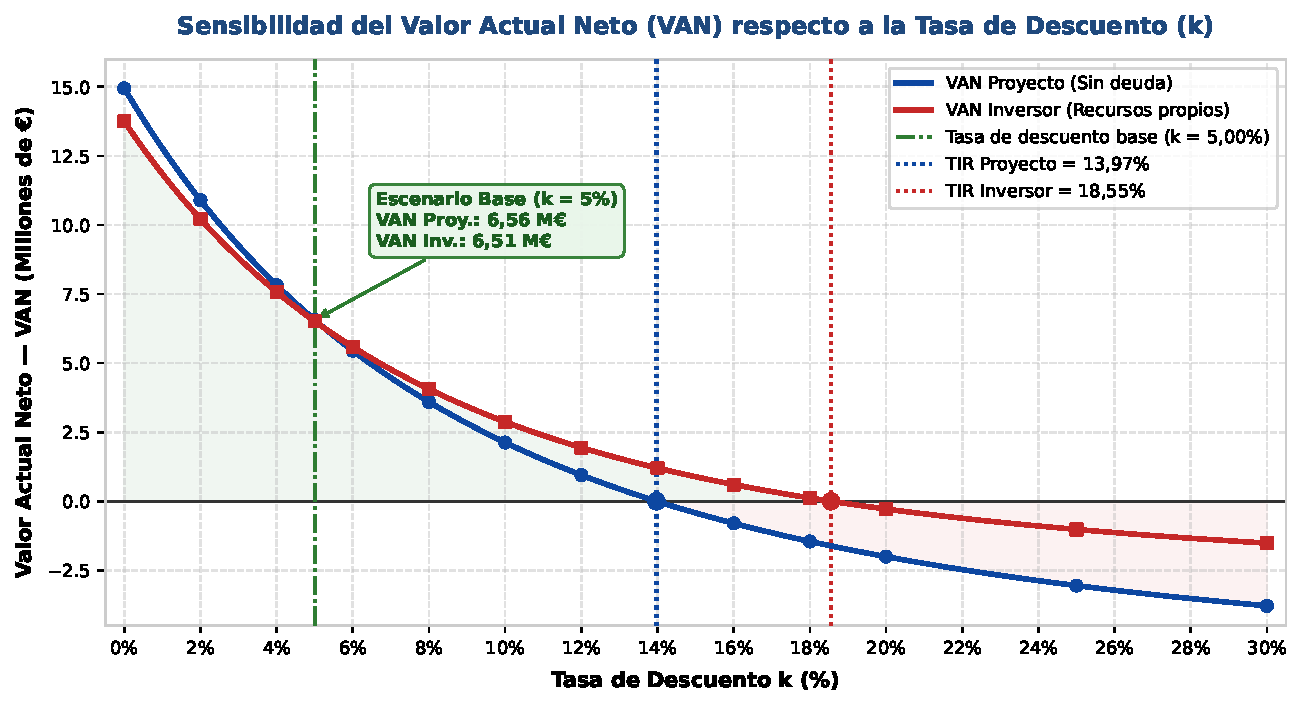
\includegraphics[width=0.92\textwidth]{figuras/sensibilidad_tasa_descuento.pdf}
\caption{Curva de sensibilidad del Valor Actual Neto del Proyecto y del Inversor respecto a la tasa de descuento $k$ (0\% a 30\%).}
\label{fig:curva_tasa}
\end{figure}

En la Tabla~\ref{tab:sensibilidad_tasa} se muestran los valores exactos obtenidos del modelo Excel, resaltando en color cian claro la fila correspondiente al escenario base de referencia ($k = 5\%$):

\begin{table}[H]
\centering
\caption{Evolución del VAN del Proyecto y del Inversor en función de la tasa de descuento $k$ (hoja \texttt{Sensibilidad}, bloque 6.1).}
\label{tab:sensibilidad_tasa}
\small
\renewcommand{\arraystretch}{1.22}
\setlength{\tabcolsep}{8pt}
\adjustbox{max width=\textwidth}{%
\begin{tabular}{>{\hspace{1.8em}}r@{\hspace{0.35em}}lrrl}
\toprule
\multicolumn{2}{c}{\textbf{Tasa de Descuento ($k$)}} & \textbf{VAN Proyecto (\euro)} & \textbf{VAN Inversor (\euro)} & \textbf{Estado de Viabilidad} \\
\midrule
0\%  &               & 14.944.834,35 & 13.746.793,21 & Viable (Flujo acumulado sin descuento) \\
2\%  &               & 10.895.050,72 & 10.211.666,35 & Viable \\
4\%  &               & 7.818.836,24  & 7.575.694,06  & Viable \\
\rowcolor{cyan!15}\textbf{5\%} & \textbf{(Base)} & \textbf{6.558.463,97} & \textbf{6.511.628,24} & \textbf{Viable (Escenario Base de Referencia)} \\
6\%  &               & 5.447.877,58  & 5.583.324,75  & Viable ($\text{VAN}_{\text{inv}} > \text{VAN}_{\text{proy}}$ para $k > 5,25\%$) \\
8\%  &               & 3.594.519,23  & 4.057.205,83  & Viable \\
10\% &               & 2.125.921,64  & 2.872.860,13  & Viable \\
12\% &               & 946.928,97    & 1.941.954,37  & Viable \\
14\% &               & -11.415,84    & 1.201.125,64  & Crítico Proyecto ($\text{TIR}_{\text{proy}} = 13,97\%$) / Viable Inversor \\
16\% &               & -799.654,32   & 604.441,53    & No viable Proyecto / Viable Inversor \\
18\% &               & -1.455.243,44 & 118.260,53    & No viable Proyecto / Límite Inversor ($\text{TIR}_{\text{inv}} = 18,55\%$) \\
20\% &               & -2.006.244,87 & -282.306,23   & No viable en ambas perspectivas ($\text{VAN} < 0$) \\
25\% &               & -3.053.637,31 & -1.020.262,24 & No viable \\
30\% &               & -3.786.042,10 & -1.515.225,82 & No viable \\
\bottomrule
\end{tabular}}
\end{table}

Como se comprueba en la Tabla~\ref{tab:sensibilidad_tasa} y en la Figura~\ref{fig:curva_tasa}, la curva azul del proyecto corta el eje horizontal ($\text{VAN}_{\text{proy}} = 0$) exactamente en $\text{TIR}_{\text{proy}} = 13,97\%$, entrando ya en terreno ligeramente negativo en el escalón del 14\% ($-11.415,84\text{ \euro}$). Por su parte, la curva roja del inversor mantiene valores positivos hasta alcanzar $\text{TIR}_{\text{inv}} = 18,55\%$, pasando de $+118.260,53\text{ \euro}$ al 18\% a $-282.306,23\text{ \euro}$ en el escalón del 20\%.

\section{Sensibilidad Multivariable y Diagrama de Tornado}
Siguiendo el guion del seminario, se analiza el impacto sobre el VAN del Inversor a la tasa base ($k = 5,00\%$, con valor de referencia $\text{VAN}_{\text{inv, base}} = 6.511.628,24\text{ \euro}$) ante variaciones individuales del $\pm 10\%$ en las tres variables operativas principales: precio de venta ($p_{\text{venta}}$), volumen de producción ($q_{\text{prod}}$) y coste anual de la materia prima ($C_{\text{MP}}$).

Para obtener de forma exacta y transparente estas variaciones (tanto analíticamente como en las celdas \texttt{F5:K14} de la hoja \texttt{Sensibilidad}), basta observar que ni las cuotas de amortización contable ni el cuadro del préstamo bancario dependen del precio de venta, del volumen producido ni del coste de la materia prima. Por consiguiente, cualquier incremento o disminución anual constante en el margen operativo bruto ($\Delta\text{EBITDA}$) modifica el flujo neto de caja de cada uno de los $N = 20$ años (tanto del proyecto como del inversor) en la cuantía neta de impuestos:
\begin{equation}
    \Delta FNC_t = (1 - t_{\text{IS}})\cdot \Delta\text{EBITDA} = (1 - 0,25)\cdot \Delta\text{EBITDA} = 0,75\cdot \Delta\text{EBITDA} \quad \forall t \in \{1,\dots,20\}
\end{equation}

Actualizando esta corriente constante de 20 años al tipo de descuento $k = 5,00\%$ mediante el factor de valor actual de una renta constante ($a_{20\rceil 0,05}$, calculado en la celda \texttt{J6} de \texttt{Sensibilidad}):
\begin{equation}
    a_{20\rceil 0,05} = \sum_{t=1}^{20} \frac{1}{(1,05)^t} = \frac{1 - (1,05)^{-20}}{0,05} = 12,46221034\text{ años equivalentes}
\end{equation}
se obtiene el \textbf{multiplicador marginal de sensibilidad del VAN respecto al EBITDA anual} (celda \texttt{J8} de \texttt{Sensibilidad}):
\begin{equation}\label{eq:multiplicador_van}
\begin{aligned}
    \mathcal{M}_{\text{VAN}} &= \frac{\partial\text{VAN}}{\partial\text{EBITDA}} = (1 - t_{\text{IS}})\cdot a_{20\rceil 0,05} \\
    &= 0,75 \times 12,46221034 = \mathbf{9,34665776\text{ \euro{} de VAN por cada 1 \euro/año de EBITDA}}
\end{aligned}
\end{equation}

Aplicando directamente la Ecuación~\eqref{eq:multiplicador_van} a cada una de las tres perturbaciones del $\pm 10\%$:
\begin{enumerate}
    \item \textbf{Variación del $\pm 10\%$ en el Precio de Venta ($p_{\text{venta}}$ de $0,9171$ a $1,1209\text{ \euro/kg}$):} Como los ingresos anuales ($2.706.372,29\text{ \euro/año}$) son linealmente proporcionales al precio unitario, un cambio del $\pm 10\%$ altera los ingresos y el EBITDA anual en $\Delta\text{EBITDA} = \pm 0,10 \times 2.706.372,29 = \pm 270.637,23\text{ \euro/año}$. La variación inducida en el VAN es:
    \begin{equation}
        \Delta\text{VAN}_{p} = \pm 270.637,229 \times 9,34665776 = \mathbf{\pm 2.529.553,56\text{ \euro}}
    \end{equation}
    situando el VAN del inversor entre $3.982.074,68\text{ \euro}$ ($-10\%$) y $9.041.181,79\text{ \euro}$ ($+10\%$), con una amplitud total de $2 \times 2.529.553,56 = \mathbf{5.059.107,11\text{ \euro}}$.
    \item \textbf{Variación del $\pm 10\%$ en Producción ($q_{\text{prod}}$ de $8,271$ a $10,109\text{ t/día}$):} En el modelo financiero del seminario (donde los costes de explotación se parametrizan de forma fija para la capacidad nominal), una fluctuación del $\pm 10\%$ en las toneladas vendidas produce exactamente la misma variación de facturación ($\Delta\text{EBITDA} = \pm 270.637,23\text{ \euro/año}$) y, por tanto, el mismo impacto de $\mathbf{\pm 2.529.553,56\text{ \euro}}$ sobre el VAN.
    \item \textbf{Variación del $\pm 10\%$ en Materia Prima ($C_{\text{MP}}$ de $675$ a $825\text{ k\euro/año}$):} Un aumento o reducción del $\pm 10\%$ sobre la partida anual de materia prima (750.000,00~\euro/año) modifica el EBITDA en sentido opuesto en $\mp 0,10 \times 750.000,00 = \mp 75.000,00\text{ \euro/año}$, lo que se traduce en una variación sobre el VAN de:
    \begin{equation}
        \Delta\text{VAN}_{\text{MP}} = \mp 75.000,00 \times 9,34665776 = \mathbf{\mp 700.999,33\text{ \euro}}
    \end{equation}
    acotando el VAN del inversor entre 5.810.628,91~\euro{} (cuando la materia prima se encarece un $+10\%$) y 7.212.627,57~\euro{} (cuando se abarata un $-10\%$), lo que arroja una amplitud total de \textbf{1.401.998,66~\euro}.
\end{enumerate}

\begin{table}[H]
\centering
\caption{Resultados del análisis de sensibilidad unidimensional ($\pm 10\%$) sobre el VAN del Inversor a $k = 5,00\%$ (hoja \texttt{Sensibilidad}, Tabla 6.2).}
\label{tab:tornado_datos}
\small
\renewcommand{\arraystretch}{1.24}
\setlength{\tabcolsep}{5.5pt}
\adjustbox{max width=\textwidth}{%
\begin{tabular}{@{}lrrrrr@{}}
\toprule
\textbf{Variable de Entrada Analizada} & \textbf{\shortstack[r]{Variación\\$|\Delta\text{VAN}|$ (\euro)}} & \textbf{\shortstack[r]{Escenario\\Desfavorable (\euro)}} & \textbf{\shortstack[r]{Escenario\\Base (\euro)}} & \textbf{\shortstack[r]{Escenario\\Favorable (\euro)}} & \textbf{\shortstack[r]{Amplitud\\Total (\euro)}} \\
\midrule
Precio de Venta ($\pm 10\%$) & 2.529.553,56 & 3.982.074,68 & 6.511.628,24 & 9.041.181,79 & \textbf{5.059.107,11} \\
Volumen de Producción ($\pm 10\%$) & 2.529.553,56 & 3.982.074,68 & 6.511.628,24 & 9.041.181,79 & \textbf{5.059.107,11} \\
Tasa de Descuento (6\% vs 4\%) & --- & 5.583.324,75 & 6.511.628,24 & 7.575.694,06 & \textbf{1.992.369,31} \\
Coste Materia Prima ($\pm 10\%$) & 700.999,33 & 5.810.628,91 & 6.511.628,24 & 7.212.627,57 & \textbf{1.401.998,66} \\
\bottomrule
\end{tabular}}
\end{table}

\begin{figure}[H]
\centering
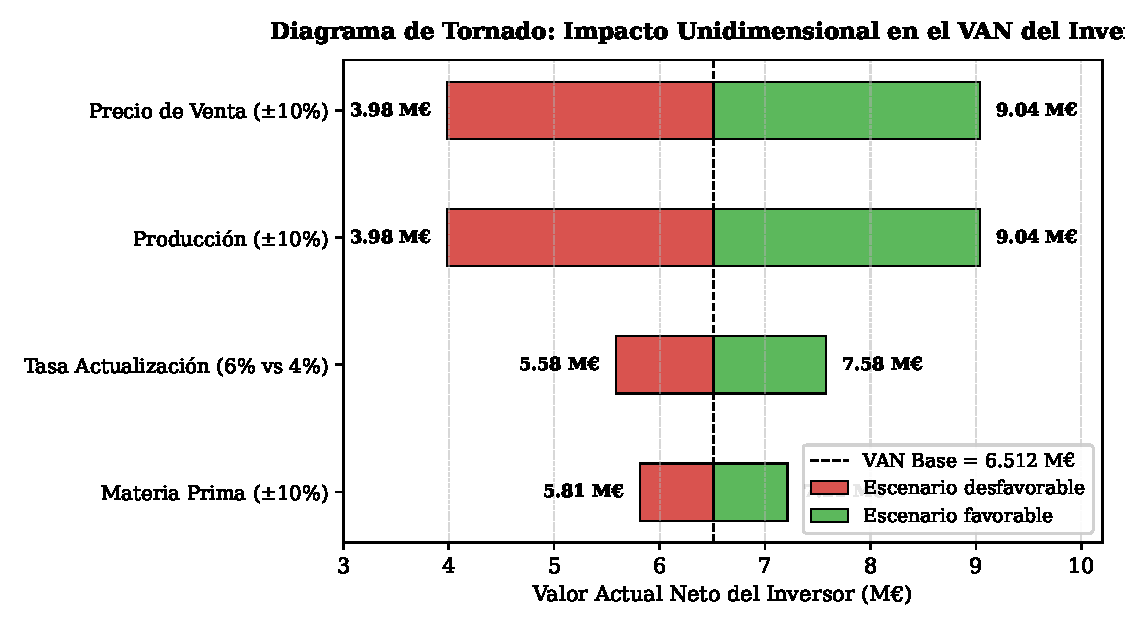
\includegraphics[width=0.92\textwidth]{figuras/diagrama_tornado_sensibilidad.pdf}
\caption{Diagrama de Tornado: comparación del impacto sobre el VAN del Inversor ante variaciones del $\pm 10\%$ en las variables críticas.}
\label{fig:diagrama_tornado}
\end{figure}

\section{Identificación de la Variable Crítica y Cálculo de Umbrales de Quiebre}
El diagrama de tornado (Figura~\ref{fig:diagrama_tornado}) pone de manifiesto que los parámetros determinantes de los ingresos (\textbf{precio de venta} y \textbf{volumen de producción}) presentan una sensibilidad 3,61 veces mayor que el coste de la materia prima ($2.706.372,29 / 750.000,00 = 3,6085$).

Para determinar analíticamente los \textbf{umbrales críticos de quiebre} que anularían el Valor Actual Neto del inversor ($\text{VAN}_{\text{inv}} = 0$ a $k = 5,00\%$), tal y como se calcula en el bloque 6.3 de la hoja \texttt{Sensibilidad} (celdas \texttt{F16:K23}), partimos de la caída máxima de EBITDA anual que puede absorber el proyecto antes de destruir valor para el accionista:
\begin{equation}
    \Delta\text{EBITDA}_{\text{crít, inv}} = -\frac{\text{VAN}_{\text{inv, base}}}{\mathcal{M}_{\text{VAN}}} = -\frac{6.511.628,24\text{ \euro}}{9,34665776\text{ años}} = \mathbf{-696.679,86\text{ \euro/año}} \quad (\text{celda \texttt{I18}})
\end{equation}
lo que supone una contracción máxima del $-50,59\%$ respecto al EBITDA anual de diseño ($1.377.072,29\text{ \euro/año}$). De esta expresión se deducen de forma inmediata los tres umbrales operativos límite:
\begin{itemize}
    \item \textbf{Precio de venta mínimo viable ($p_{\text{mín}}$):} Para que la facturación anual se reduzca en $696.679,86\text{ \euro/año}$ manteniendo constante la producción, los ingresos deben contraerse en un porcentaje crítico de:
    \begin{equation}
        \Delta\%_{\text{ingresos, crít}} = \frac{-696.679,86\text{ \euro/año}}{2.706.372,29\text{ \euro/año}} = \mathbf{-25,74\%} \quad (\text{celda \texttt{H19}})
    \end{equation}
    lo que fija el precio de venta mínimo admisible en:
    \begin{equation}
        p_{\text{mín}} = 1,019\text{ \euro/kg} \times (1 - 0,257422) = \mathbf{0,7567\text{ \euro/kg}} \quad (\text{celda \texttt{I19}})
    \end{equation}
    \item \textbf{Volumen de producción mínimo viable ($q_{\text{mín}}$):} Análogamente, a precio constante de $1,019\text{ \euro/kg}$, la planta puede soportar una caída del $\mathbf{-25,74\%}$ en su ritmo productivo antes de entrar en $\text{VAN}_{\text{inv}} < 0$:
    \begin{equation}
        q_{\text{mín}} = 9,19\text{ t/día} \times (1 - 0,257422) = \mathbf{6,824\text{ t/día}} \quad (1.972,22\text{ t/año, celdas \texttt{I20:I21}})
    \end{equation}
    \item \textbf{Coste máximo admisible de la materia prima ($C_{\text{MP, máx}}$):} Para que el encarecimiento de la materia prima consuma por sí solo el colchón de $696.679,86\text{ \euro/año}$ de EBITDA, la factura anual de materias primas tendría que incrementarse en:
    \begin{equation}
    \begin{aligned}
        \Delta\%_{\text{MP, crít}} &= \frac{+696.679,86\text{ \euro/año}}{750.000,00\text{ \euro/año}} = \mathbf{+92,89\%} \\
        \implies C_{\text{MP, máx}} &= 750.000,00 + 696.679,86 = \mathbf{1.446.679,86\text{ \euro/año}}
    \end{aligned}
    \end{equation}
    (recogido en las celdas \texttt{H22} e \texttt{I22} de la hoja \texttt{Sensibilidad}).
    \item \textbf{Tasa de descuento límite ($\text{TIR}$):} Respecto al coste del capital, el proyecto puro soporta tasas de actualización de hasta el $\mathbf{13,97\%}$ y el inversor apalancado de hasta el $\mathbf{18,55\%}$ antes de que sus respectivos VAN pasen a ser negativos.
\end{itemize}

\chapter{Conclusiones y Recomendación Técnica}

\section{Recomendación Tras el Análisis de Sensibilidad}
A partir de los resultados obtenidos en el modelo económico-financiero y en el estudio de sensibilidad paramétrica, se formulan las siguientes conclusiones ejecutivas:
\begin{enumerate}
    \item \textbf{Dictamen favorable de inversión:} Se recomienda \textbf{aprobar la ejecución del proyecto}. Tanto los activos de la planta ($\text{VAN}_{\text{proy}} = 6,56\text{ M\euro}$, $\text{TIR}_{\text{proy}} = 13,97\%$, $\text{PRI}_{\text{proy}} = 6,58\text{ años}$) como los recursos propios de los promotores ($\text{VAN}_{\text{inv}} = 6,51\text{ M\euro}$, $\text{TIR}_{\text{inv}} = 18,55\%$, $\text{PRI}_{\text{inv}} = 5,71\text{ años}$) superan ampliamente el coste de oportunidad del capital ($k = 5,00\%$).
    \item \textbf{Conveniencia de la financiación bancaria:} El préstamo francés por el 49,50\% de la inversión ($3.769.425,00\text{ \euro}$ al 7,00\% a 10 años) resulta ventajoso para los accionistas. Dado que la TIR del proyecto ($13,97\%$) casi duplica el coste nominal de la deuda ($7,00\%$) y los intereses generan un escudo fiscal de $399.347,05\text{ \euro}$, el apalancamiento eleva la TIR del inversor en $+4,58\text{ puntos porcentuales}$ y adelanta en $0,87\text{ años}$ la recuperación del capital.
    \item \textbf{Gestión de riesgos sobre variables críticas:} Siendo el precio de venta y el volumen de producción los factores más sensibles ($\pm 2,53\text{ M\euro}$ de variación en el VAN por cada $\pm 10\%$), la estrategia durante los primeros años debe asegurar acuerdos comerciales por encima del umbral crítico de $0,7567\text{ \euro/kg}$ y mantener un programa preventivo sobre la maquinaria principal ($6,50\text{ M\euro}$) para garantizar los 289 días de operación anual (por encima del límite de $6,824\text{ t/día}$).
\end{enumerate}

\section{Valoración Final}
El estudio demuestra que el diseño técnico y la estructuración financiera forman un sistema acoplado. La correcta contabilización de los escalones de amortización (años 1--10, 11--15 y 16--20) y del escudo fiscal confirma que la planta genera $1.156.512,55\text{ \euro/año}$ de flujo operativo frente a $536.681,32\text{ \euro/año}$ de cuota bancaria, garantizando una solvencia sólida durante los veinte años de vida útil.

\chapter*{Declaración sobre el Uso de Inteligencia Artificial Generativa}
\addcontentsline{toc}{chapter}{Declaración sobre el Uso de Inteligencia Artificial Generativa}

En cumplimiento de las directrices de integridad académica y transparencia de la Universidad de Granada (UGR) para la elaboración de trabajos técnicos y memorias de grado, el autor declara el uso de herramientas de Inteligencia Artificial Generativa (\textit{Claude} de Anthropic y \textit{Gemini} de Google) exclusivamente como asistente de apoyo durante la fase final de edición y revisión del presente Estudio Económico y Financiero.

Todos los fundamentos teóricos, el planteamiento económico-financiero, la selección de parámetros y la elaboración íntegra de los cálculos han sido realizados por el autor. La asistencia de estas herramientas se ha limitado estrictamente a:
\begin{enumerate}
    \item \textbf{Estética y maquetación del documento:} Mejora de la presentación visual, homogeneización tipográfica de tablas y figuras, y ajuste de márgenes y formato general de la memoria.
    \item \textbf{Auditoría y comprobación de cálculos:} Verificación cruzada de los resultados numéricos, fórmulas de actualización de flujos de caja, cuadros de amortización e indicadores de rentabilidad ya desarrollados por el autor, con el fin de garantizar la ausencia de errores aritméticos o de transcripción entre la hoja de cálculo y la memoria.
    \item \textbf{Revisión ortotipográfica y de estilo:} Corrección gramatical y pulido de la redacción técnica para asegurar la claridad expositiva del texto.
\end{enumerate}

El autor asume la plena responsabilidad sobre la exactitud, originalidad y rigor académico del contenido final de esta memoria.

\vspace{4.5em}
\noindent\begin{tabular*}{\linewidth}{@{}l @{\extracolsep{\fill}} r@{}}
\textbf{Firma del Estudiante:} & \textbf{Fecha:} 13/11/2026 \\[2.8em]
\hline
\rule{0pt}{1.4em}Christian Pérez Hita & \\
DNI: 49559419P &
\end{tabular*}

\begin{thebibliography}{9}
\addcontentsline{toc}{chapter}{Bibliografía}

\bibitem{seminario_ogp}
Departamento de Ingeniería Química (2026). \textit{Seminario: Elaboración del Estudio Económico-Financiero de una Planta Industrial}. Asignatura: Organización y Gestión de Proyectos, Grado en Ingeniería Química, Universidad de Granada.

\bibitem{brealey_myers}
Brealey, R. A., Myers, S. C. y Allen, F. (2020). \textit{Principios de Finanzas Corporativas} (13.ª ed.). McGraw-Hill Interamericana.

\bibitem{sinnott_towler}
Towler, G. y Sinnott, R. (2021). \textit{Chemical Engineering Design: Principles, Practice and Economics of Plant and Process Design} (3.ª ed.). Butterworth-Heinemann / Elsevier.

\bibitem{ley_is}
Jefatura del Estado (2014). \textit{Ley 27/2014, de 27 de noviembre, del Impuesto sobre Sociedades} (Tipo general de gravamen del 25\% y tablas oficiales de coeficientes de amortización lineal, art. 12). Boletín Oficial del Estado (BOE núm. 288).

\bibitem{anthropic_claude}
Anthropic (2026). \textit{Claude (Familia de modelos Claude 4)} [Modelo de lenguaje de gran tamaño]. Asistente en estética documental, auditoría de cálculos y revisión de estilo técnico. Disponible en: \url{https://www.anthropic.com}.

\bibitem{google_gemini}
Google DeepMind (2026). \textit{Gemini} [Modelo de inteligencia artificial multimodal]. Asistente en estética documental, auditoría de cálculos y revisión de estilo técnico. Disponible en: \url{https://gemini.google.com}.

\end{thebibliography}

\end{document}
